\chapterimage{head2.png} % Chapter heading image
\chapter{EM Algorithm}

\section{The General EM Algorithm}
\begin{definition}[The joint probability]
    \begin{equation}
        p(\textbf{x}, \textbf{y})= p(x_0)\prod_{t=1}^{T} p(x_{t}|x_{t-1}) p(y_t|x_t)
    \end{equation}
    \begin{center}
        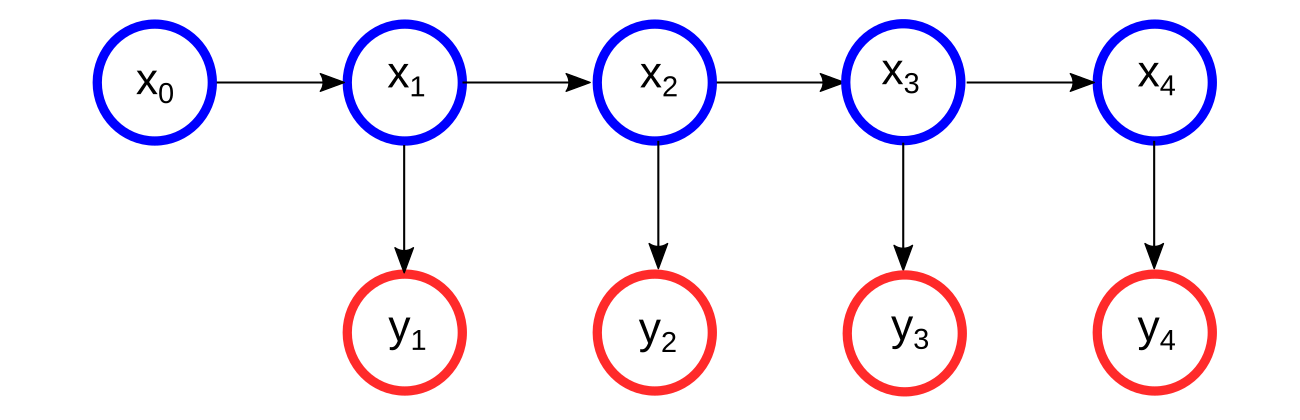
\includegraphics[scale=0.6]{ch2/four_states_ex.png}   
    \end{center}
In this example
    \begin{equation}
    \begin{split}
        p(\textbf{x}, \textbf{y})= &[p(x_0) p(x_1|x_0) p(y_1|x_1)] [p(x_2|x_1) p(y_2|x_2)]  [p(x_3|x_2) p(y_3|x_3)] \\
        &[p(x_4|x_3) p(y_4|x_4)]
    \end{split}
    \end{equation}
\end{definition}

\begin{definition}[The likelihood functional]
\begin{equation}
    L[\theta] = p(\textbf{y};\theta) = \int d\textbf{x}p(\textbf{x}, \textbf{y})
\end{equation}
\end{definition}

\begin{definition}[The log-likelihood functional]
\begin{equation}
    l[\theta] = \ln{(\int d\textbf{x}p(\textbf{x}, \textbf{y}))}
\end{equation}
\end{definition}

\begin{definition}[Solve Euler-Lagrange equation]
Maximization for the optimal parameter set requires taking derivatives of the log-likelihood functional and solves the resulting Euler-Lagrange equation:
\begin{equation}
        \frac{\partial l[\theta]}{\partial \theta} = \frac{\partial}{\partial \theta} \ln{(\int d\textbf{x}p(\textbf{x}, \textbf{y}))} = 0
\end{equation}
We can further get
\begin{equation}
    \frac{\partial l[\theta]}{\partial \theta} =  \frac{\partial \ln{L[\theta]}}{\partial \theta} = \frac{1}{L[\theta]}\frac{\partial L[\theta]}{\partial \theta}
\end{equation}
Because we need to do maximization according to previous step($k$), we want to solve the
following equation
\begin{equation}
    0 = \frac{\partial l^k[\theta]}{\partial \theta} = \frac{1}{L^k[\theta]}\frac{\partial L^k[\theta]}{\partial \theta}
\end{equation}
And we can express the likelihood functional as
\begin{equation}
    L^k[\theta] = p(\textbf{y}) = \sum_{\tau=0}^{T-1} \left<\alpha^k_{t_{\tau}}\right|  e^{-\textbf{H} \Delta t} \left|\beta^k_{t_{\tau+1}}\right>
\end{equation}
Therefore, the maximization problem becomes to solve
\begin{equation}
    0 =  \frac{\partial l^k[\theta]}{\partial \theta} = \frac{1}{L^k[\theta]} \sum_{\tau=0}^{T-1} \frac{\partial}{\partial \theta} \left<\alpha^k_{t_{\tau}}\right|  e^{-\textbf{H} \Delta t} \left|\beta^k_{t_{\tau+1}}\right>
\end{equation}
\end{definition}

\section{The expected log of the complete likelihood}
\begin{definition}[$\left<\alpha^k_{t_{0}}\right|  e^{-\textbf{H} \Delta t} \left|\beta^k_{t_{1}}\right>$]
\begin{equation}
    \left< \alpha_{t_0} | e^{-\textbf{H}\Delta t} | \beta_{t_1} \right> = \int p(x_0) p(x_1|x_0) p(y_2,y_3,y_4|x_1) dx_1= p(x_0,y_2,y_3,y_4)
\end{equation}
    \begin{center}
        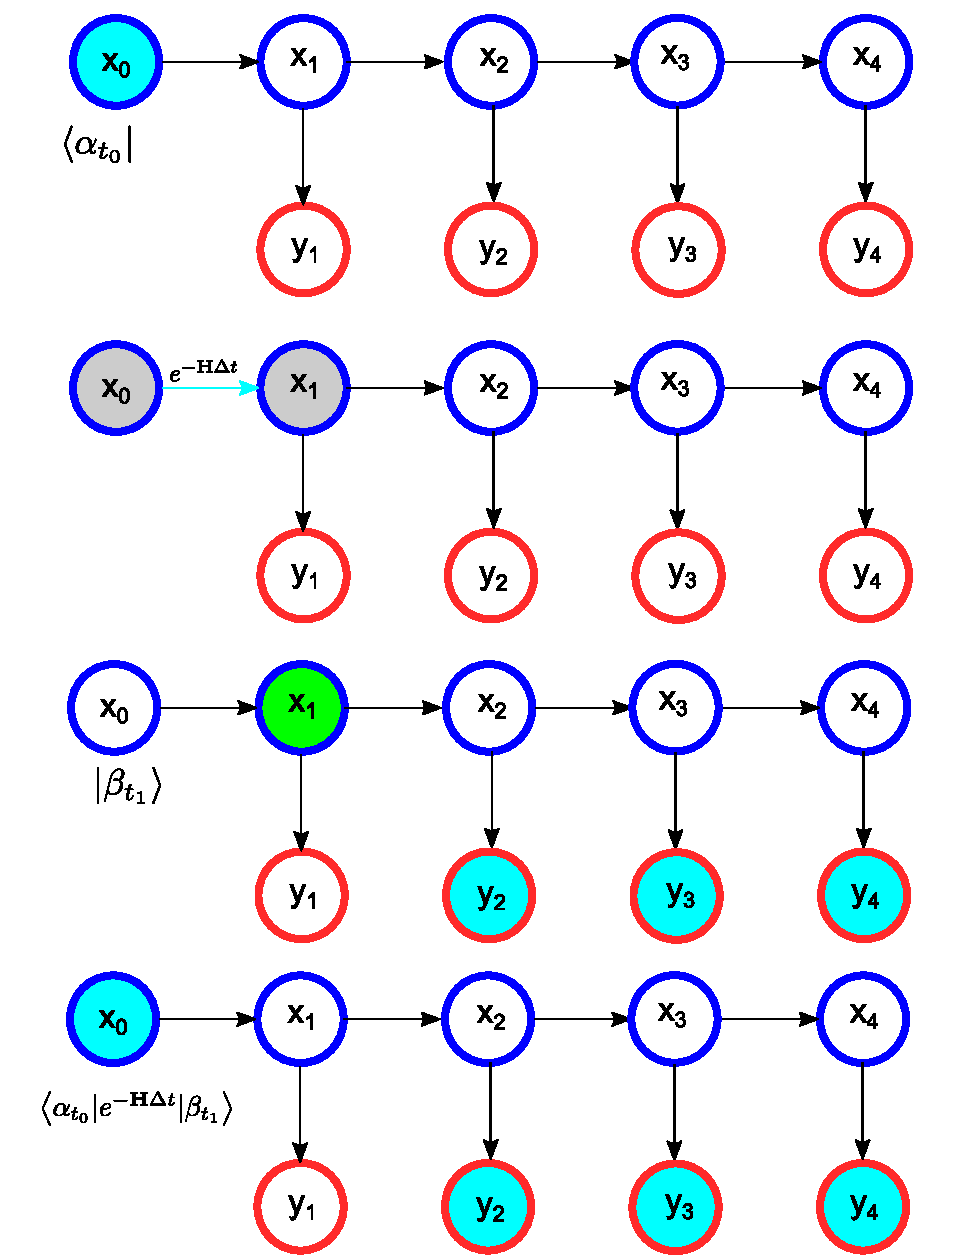
\includegraphics[scale=0.25]{ch4/alpha_t0_e_beta_t1.pdf}   
    \end{center}
\end{definition}

\begin{definition}[$\left<\alpha^k_{t_{1}}\right|  e^{-\textbf{H} \Delta t} \left|\beta^k_{t_{2}}\right>$]
\begin{equation}
    \left< \alpha_{t_1} | e^{-\textbf{H}\Delta t} | \beta_{t_2} \right> = \int p(x_1,y_1) p(x_2|x_1) p(y_3,y_4|x_2) dx_2= p(x_1,y_1,y_3,y_4)
\end{equation}
\begin{center}
    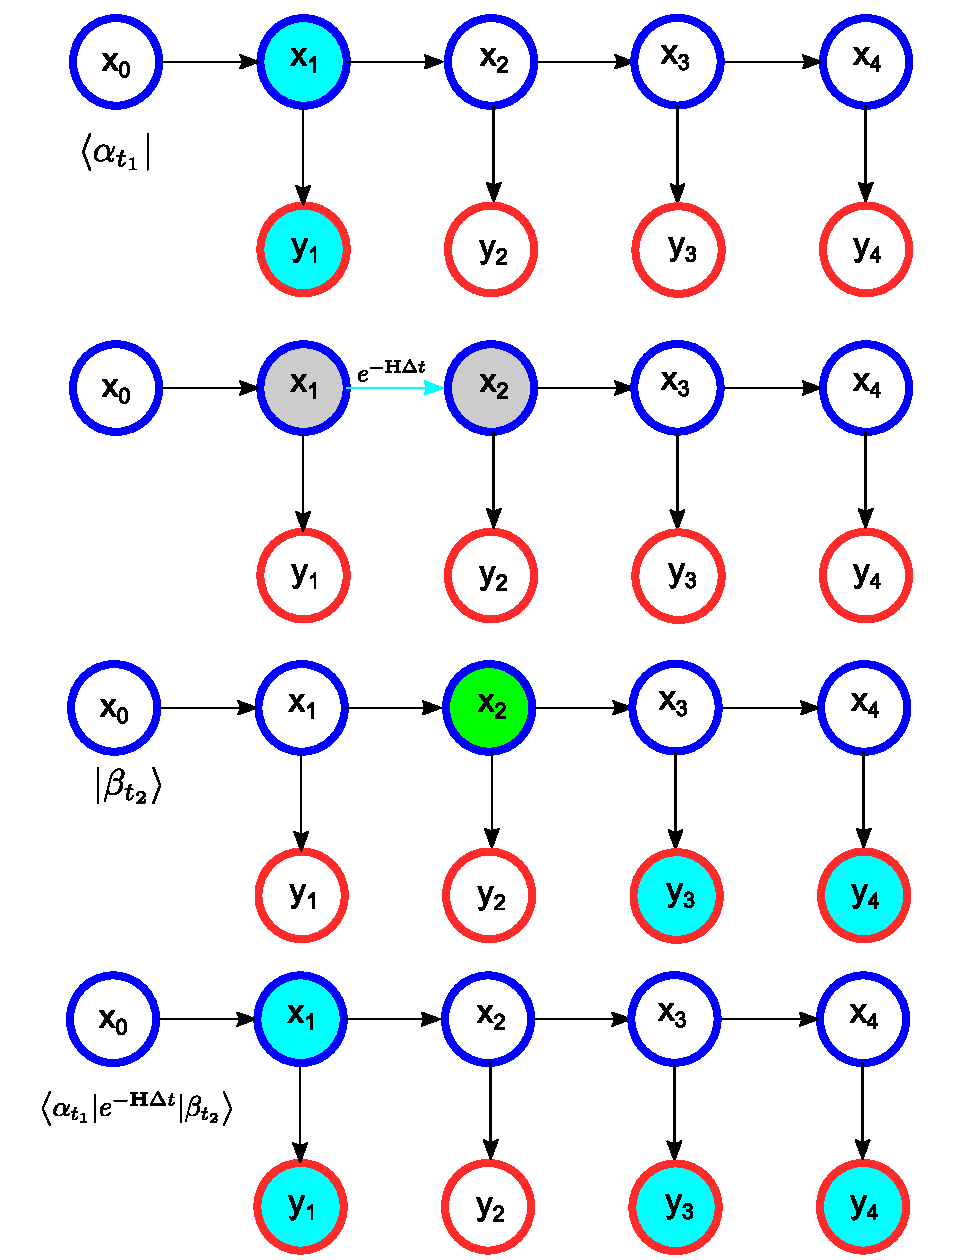
\includegraphics[scale=0.35]{ch4/alpha_t1_e_beta_t2.pdf}   
\end{center}
\end{definition}

\begin{definition}[$\left<\alpha^k_{t_{2}}\right|  e^{-\textbf{H} \Delta t} \left|\beta^k_{t_{3}}\right>$]
\begin{equation}
    \left< \alpha_{t_2} | e^{-\textbf{H}\Delta t} | \beta_{t_3} \right> = \int p(x_2,y_1,y_2) p(x_3|x_2) p(y_4|x_3) dx_3= p(x_2,y_1,y_2,y_4)
\end{equation}
\begin{center}
    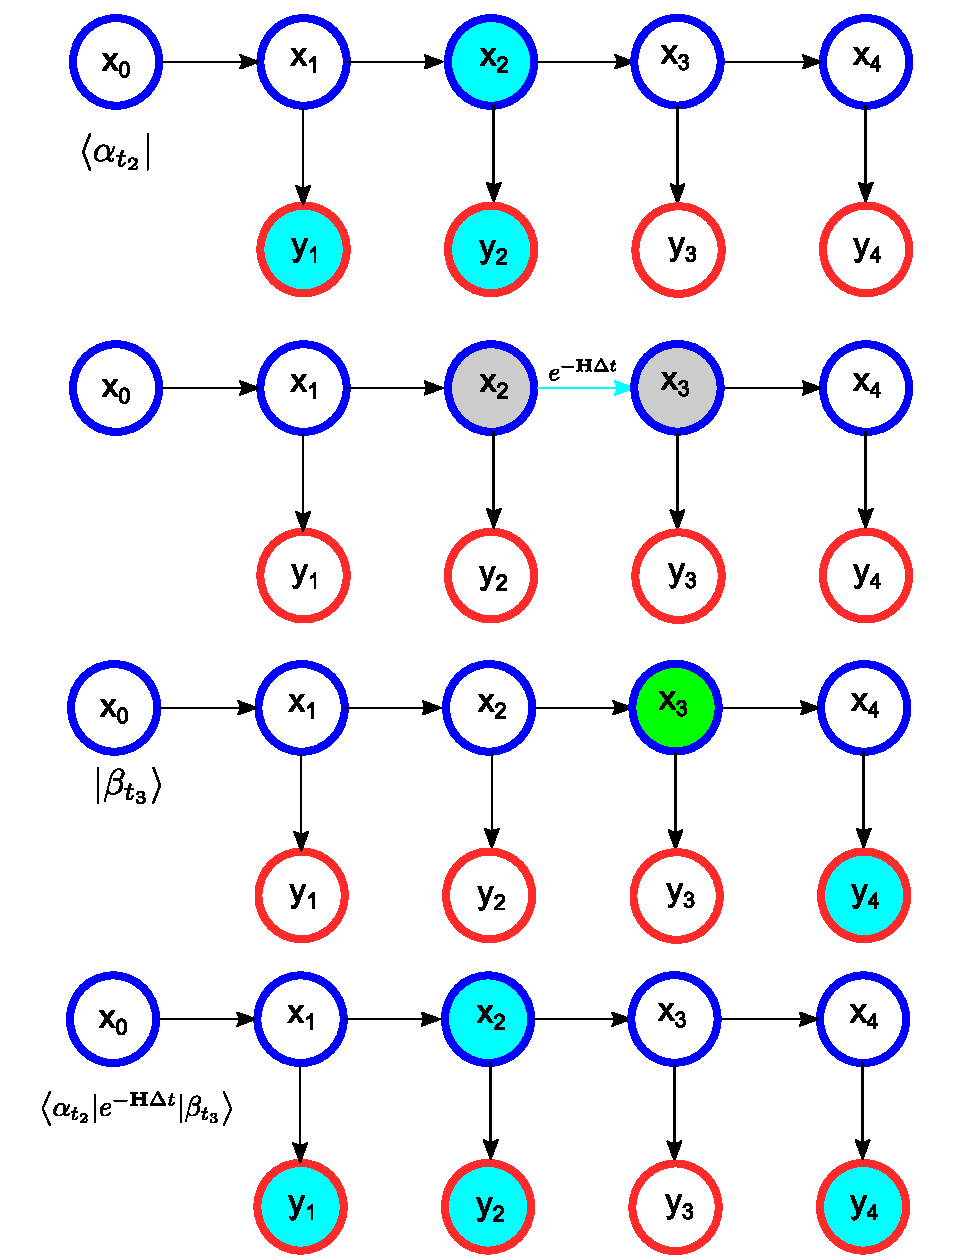
\includegraphics[scale=0.35]{ch4/alpha_t2_e_beta_t3.pdf}   
\end{center}
\end{definition}

\begin{definition}[$\left<\alpha^k_{t_{3}}\right|  e^{-\textbf{H} \Delta t} \left|\beta^k_{t_{4}}\right>$]
\begin{equation}
    \left< \alpha_{t_3} | e^{-\textbf{H}\Delta t} | \beta_{t_4} \right> = \int p(x_3,y_1,y_2,y_3) p(x_4|x_3) dx_4= p(x_3,y_1,y_2,y_3)
\end{equation}
\begin{center}
    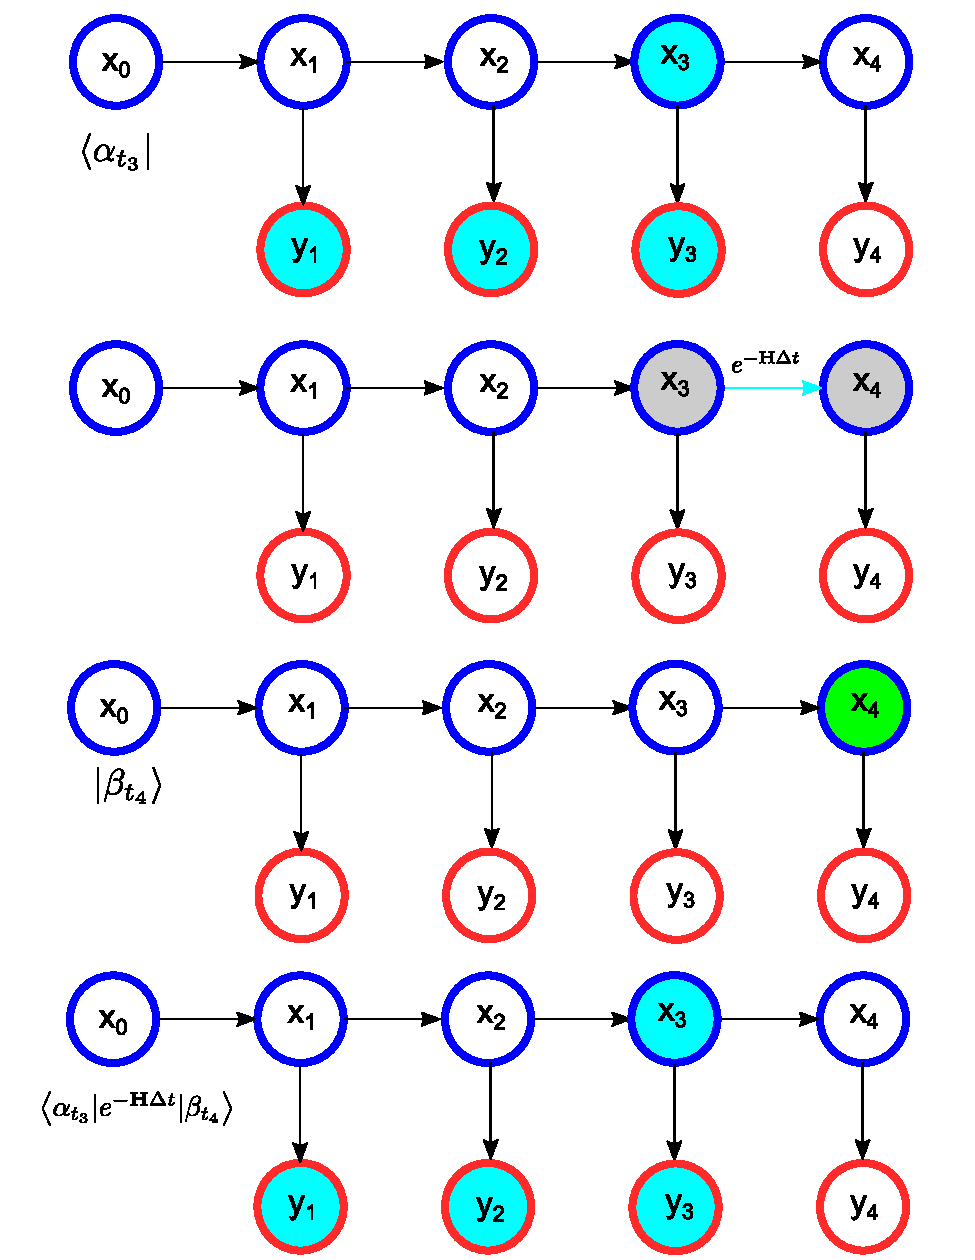
\includegraphics[scale=0.25]{ch4/alpha_t3_e_beta_t4.pdf}   
\end{center}
\end{definition}

\section{Update the equilibrium probability density}
\begin{definition}
    The basis functions in Def.(\ref{basisfunctions}) were used to update
\begin{align}
    p_{\rm eq}^{k+1}(x) &=\mathbb{E}^k_{X|Y} \left[ \delta(x-X) \right] \\
    &= p^k_{\rm{eq}}(x) \sum_{i,j} \mathbb{E}^k_{X|Y}[a_ib_j] \phi_i(x)\phi_j(x) \\
    &= \sum_{i,j} \psi_i(x) \mathbb{E}^k_{X|Y}[a_ib_j] \psi_j(x).
\end{align}
\end{definition}

\begin{definition}[Update from matrix multiplication]
\begin{align}
    p_{\rm eq}^{k+1}(x) = \mathrm{diag}(\Psi \mathbb{E}^k_{X|Y}[a_ib_j] \Psi^{\dagger})
\end{align}
\end{definition}

\begin{example}[$N_v=3$] In the matrix multiplication, I abbreviate $\mathbb{E}^k_{X|Y}[a_ib_j]$ as $a_ib_j$, and the grids are set like the bottom figure. We will show
\begin{align*}
    p_{\rm eq}^{k+1}(x) &=\sum_{i,j} \psi_i(x) \mathbb{E}^k_{X|Y}[a_ib_j] \psi_j(x) \\
    &= \mathrm{diag}(\Psi \mathbb{E}^k_{X|Y}[a_ib_j] \Psi^{\dagger})
\end{align*}
\begin{center}
    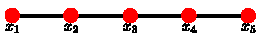
\includegraphics[scale=1.5]{ch4/ex1_grids.pdf}   
\end{center}
\begin{align*} 
&\Psi \mathbb{E}^k_{X|Y}[a_ib_j] \Psi^{\dagger} = \\
&\begin{bmatrix}
    \psi_1(x_1) & \psi_2(x_1) & \psi_3(x_1)  \\
    \psi_1(x_2) & \psi_2(x_2) & \psi_3(x_2) \\
    \psi_1(x_3) & \psi_2(x_3) & \psi_3(x_3)  \\
    \psi_1(x_4) & \psi_2(x_4) & \psi_3(x_4)  \\
    \psi_1(x_5) & \psi_2(x_5) & \psi_3(x_5)  
\end{bmatrix}
\begin{bmatrix}
    a_1 b_1 & a_1 b_2 & a_1 b_3  \\
    a_2 b_1 & a_2 b_2 & a_2 b_3 \\
    a_3 b_1 & a_3 b_2 & a_3 b_3
\end{bmatrix}
\begin{bmatrix}
    \psi_1(x_1) & \psi_1(x_2) & \psi_1(x_3) & \psi_1(x_4) & \psi_1(x_5) \\
    \psi_2(x_1) & \psi_2(x_2) & \psi_2(x_3) & \psi_2(x_4) & \psi_2(x_5) \\
    \psi_3(x_1) & \psi_3(x_2) & \psi_3(x_3) & \psi_3(x_4) & \psi_3(x_5) 
\end{bmatrix} \\
&=\begin{bmatrix}
    \sum_{i=1}^{3}a_i b_1 \psi_i(x_1) & \sum_{i=1}^{3}a_i b_2 \psi_i(x_1) & \sum_{i=1}^{3}a_i b_3 \psi_i(x_1) \\
    \sum_{i=1}^{3}a_i b_1 \psi_i(x_2) & \sum_{i=1}^{3}a_i b_2 \psi_i(x_2) & \sum_{i=1}^{3}a_i b_3 \psi_i(x_2) \\
    \sum_{i=1}^{3}a_i b_1 \psi_i(x_3) & \sum_{i=1}^{3}a_i b_2 \psi_i(x_3) & \sum_{i=1}^{3}a_i b_3 \psi_i(x_3) \\
    \sum_{i=1}^{3}a_i b_1 \psi_i(x_4) & \sum_{i=1}^{3}a_i b_2 \psi_i(x_4) & \sum_{i=1}^{3}a_i b_3 \psi_i(x_4) \\
    \sum_{i=1}^{3}a_i b_1 \psi_i(x_5) & \sum_{i=1}^{3}a_i b_2 \psi_i(x_5) & \sum_{i=1}^{3}a_i b_3 \psi_i(x_5) 
\end{bmatrix}\\
&\begin{bmatrix}
    \psi_1(x_1) & \psi_1(x_2) & \psi_1(x_3) & \psi_1(x_4) & \psi_1(x_5) \\
    \psi_2(x_1) & \psi_2(x_2) & \psi_2(x_3) & \psi_2(x_4) & \psi_2(x_5) \\
    \psi_3(x_1) & \psi_3(x_2) & \psi_3(x_3) & \psi_3(x_4) & \psi_3(x_5) 
\end{bmatrix}\\
&=
\begin{bmatrix}
\sum_{j=1}^{3} b_j \psi_j(x_1) \sum_{i=1}^{3}a_i \psi_i(x_1) &  \sum_{j=1}^{3} b_j \psi_j(x_2) \sum_{i=1}^{3}a_i \psi_i(x_1) &
\cdots & \sum_{j=1}^{3} b_j \psi_j(x_5) \sum_{i=1}^{3}a_i \psi_i(x_1) \\
\sum_{j=1}^{3} b_j \psi_j(x_1) \sum_{i=1}^{3}a_i \psi_i(x_2) &  \sum_{j=1}^{3} b_j \psi_j(x_2) \sum_{i=1}^{3}a_i \psi_i(x_2) &
\cdots & \sum_{j=1}^{3} b_j \psi_j(x_5) \sum_{i=1}^{3}a_i \psi_i(x_2) \\
\sum_{j=1}^{3} b_j \psi_j(x_1) \sum_{i=1}^{3}a_i \psi_i(x_3) &  \sum_{j=1}^{3} b_j \psi_j(x_2) \sum_{i=1}^{3}a_i \psi_i(x_3) &
\cdots & \sum_{j=1}^{3} b_j \psi_j(x_5) \sum_{i=1}^{3}a_i \psi_i(x_3) \\
\sum_{j=1}^{3} b_j \psi_j(x_1) \sum_{i=1}^{3}a_i \psi_i(x_4) &  \sum_{j=1}^{3} b_j \psi_j(x_2) \sum_{i=1}^{3}a_i \psi_i(x_4) &
\cdots & \sum_{j=1}^{3} b_j \psi_j(x_5) \sum_{i=1}^{3}a_i \psi_i(x_4) \\
\sum_{j=1}^{3} b_j \psi_j(x_1) \sum_{i=1}^{3}a_i \psi_i(x_5) &  \sum_{j=1}^{3} b_j \psi_j(x_2) \sum_{i=1}^{3}a_i \psi_i(x_5) &
\cdots & \sum_{j=1}^{3} b_j \psi_j(x_5) \sum_{i=1}^{3}a_i \psi_i(x_5)
\end{bmatrix}
\end{align*}
\end{example}

\section{EM Test}
\begin{center}
    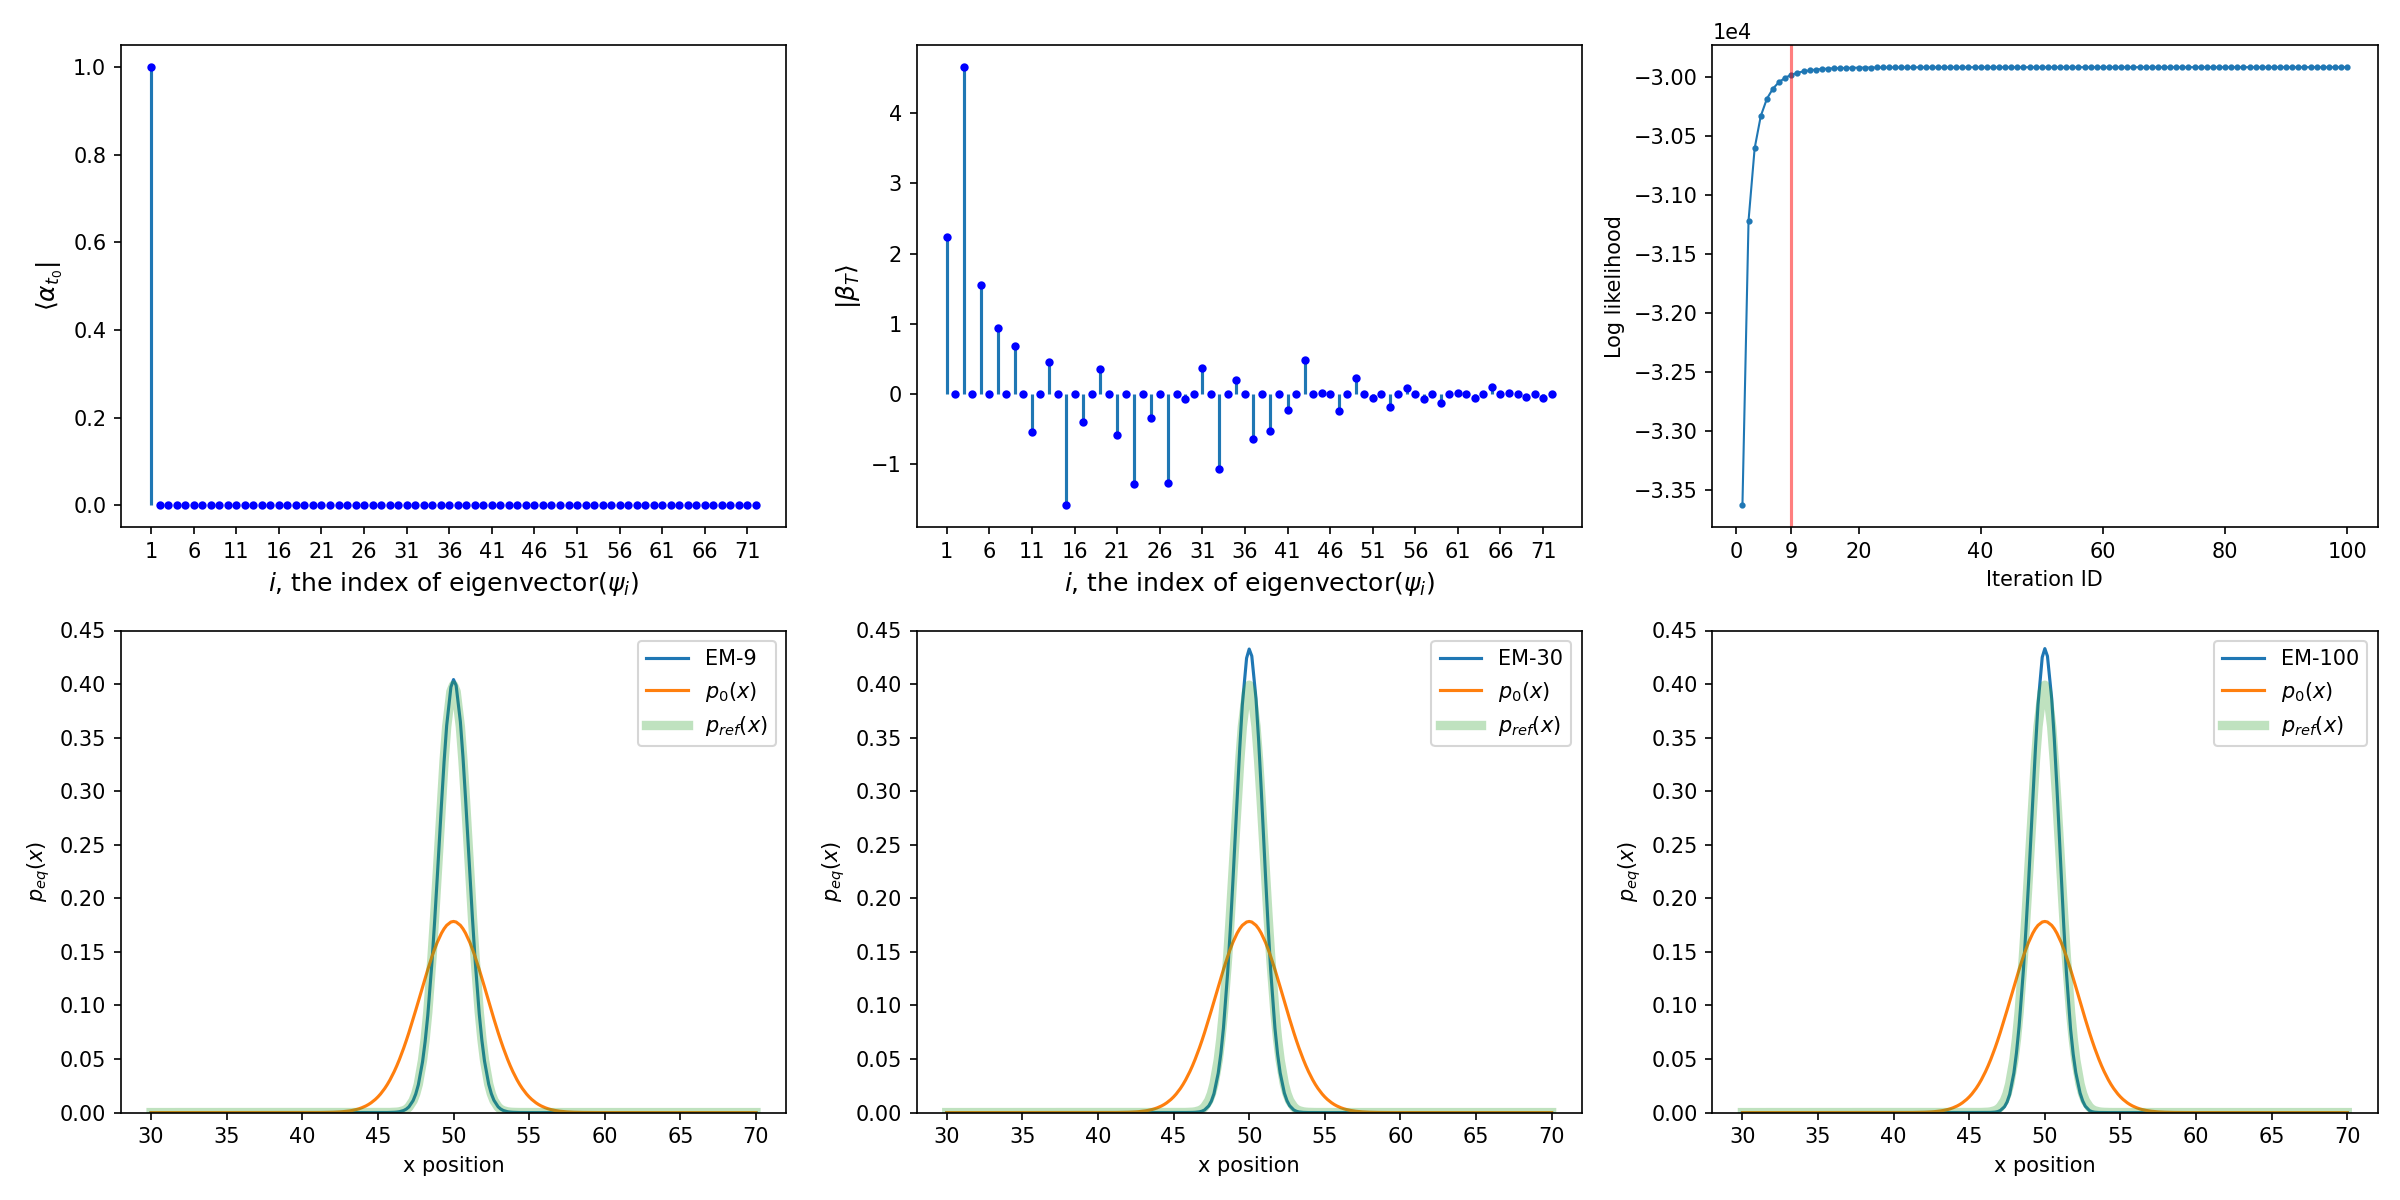
\includegraphics[scale=0.36]{ch4/forward_backward_v2.png}   
\end{center}

\subsection{Initial Guess Test}
\begin{center}
    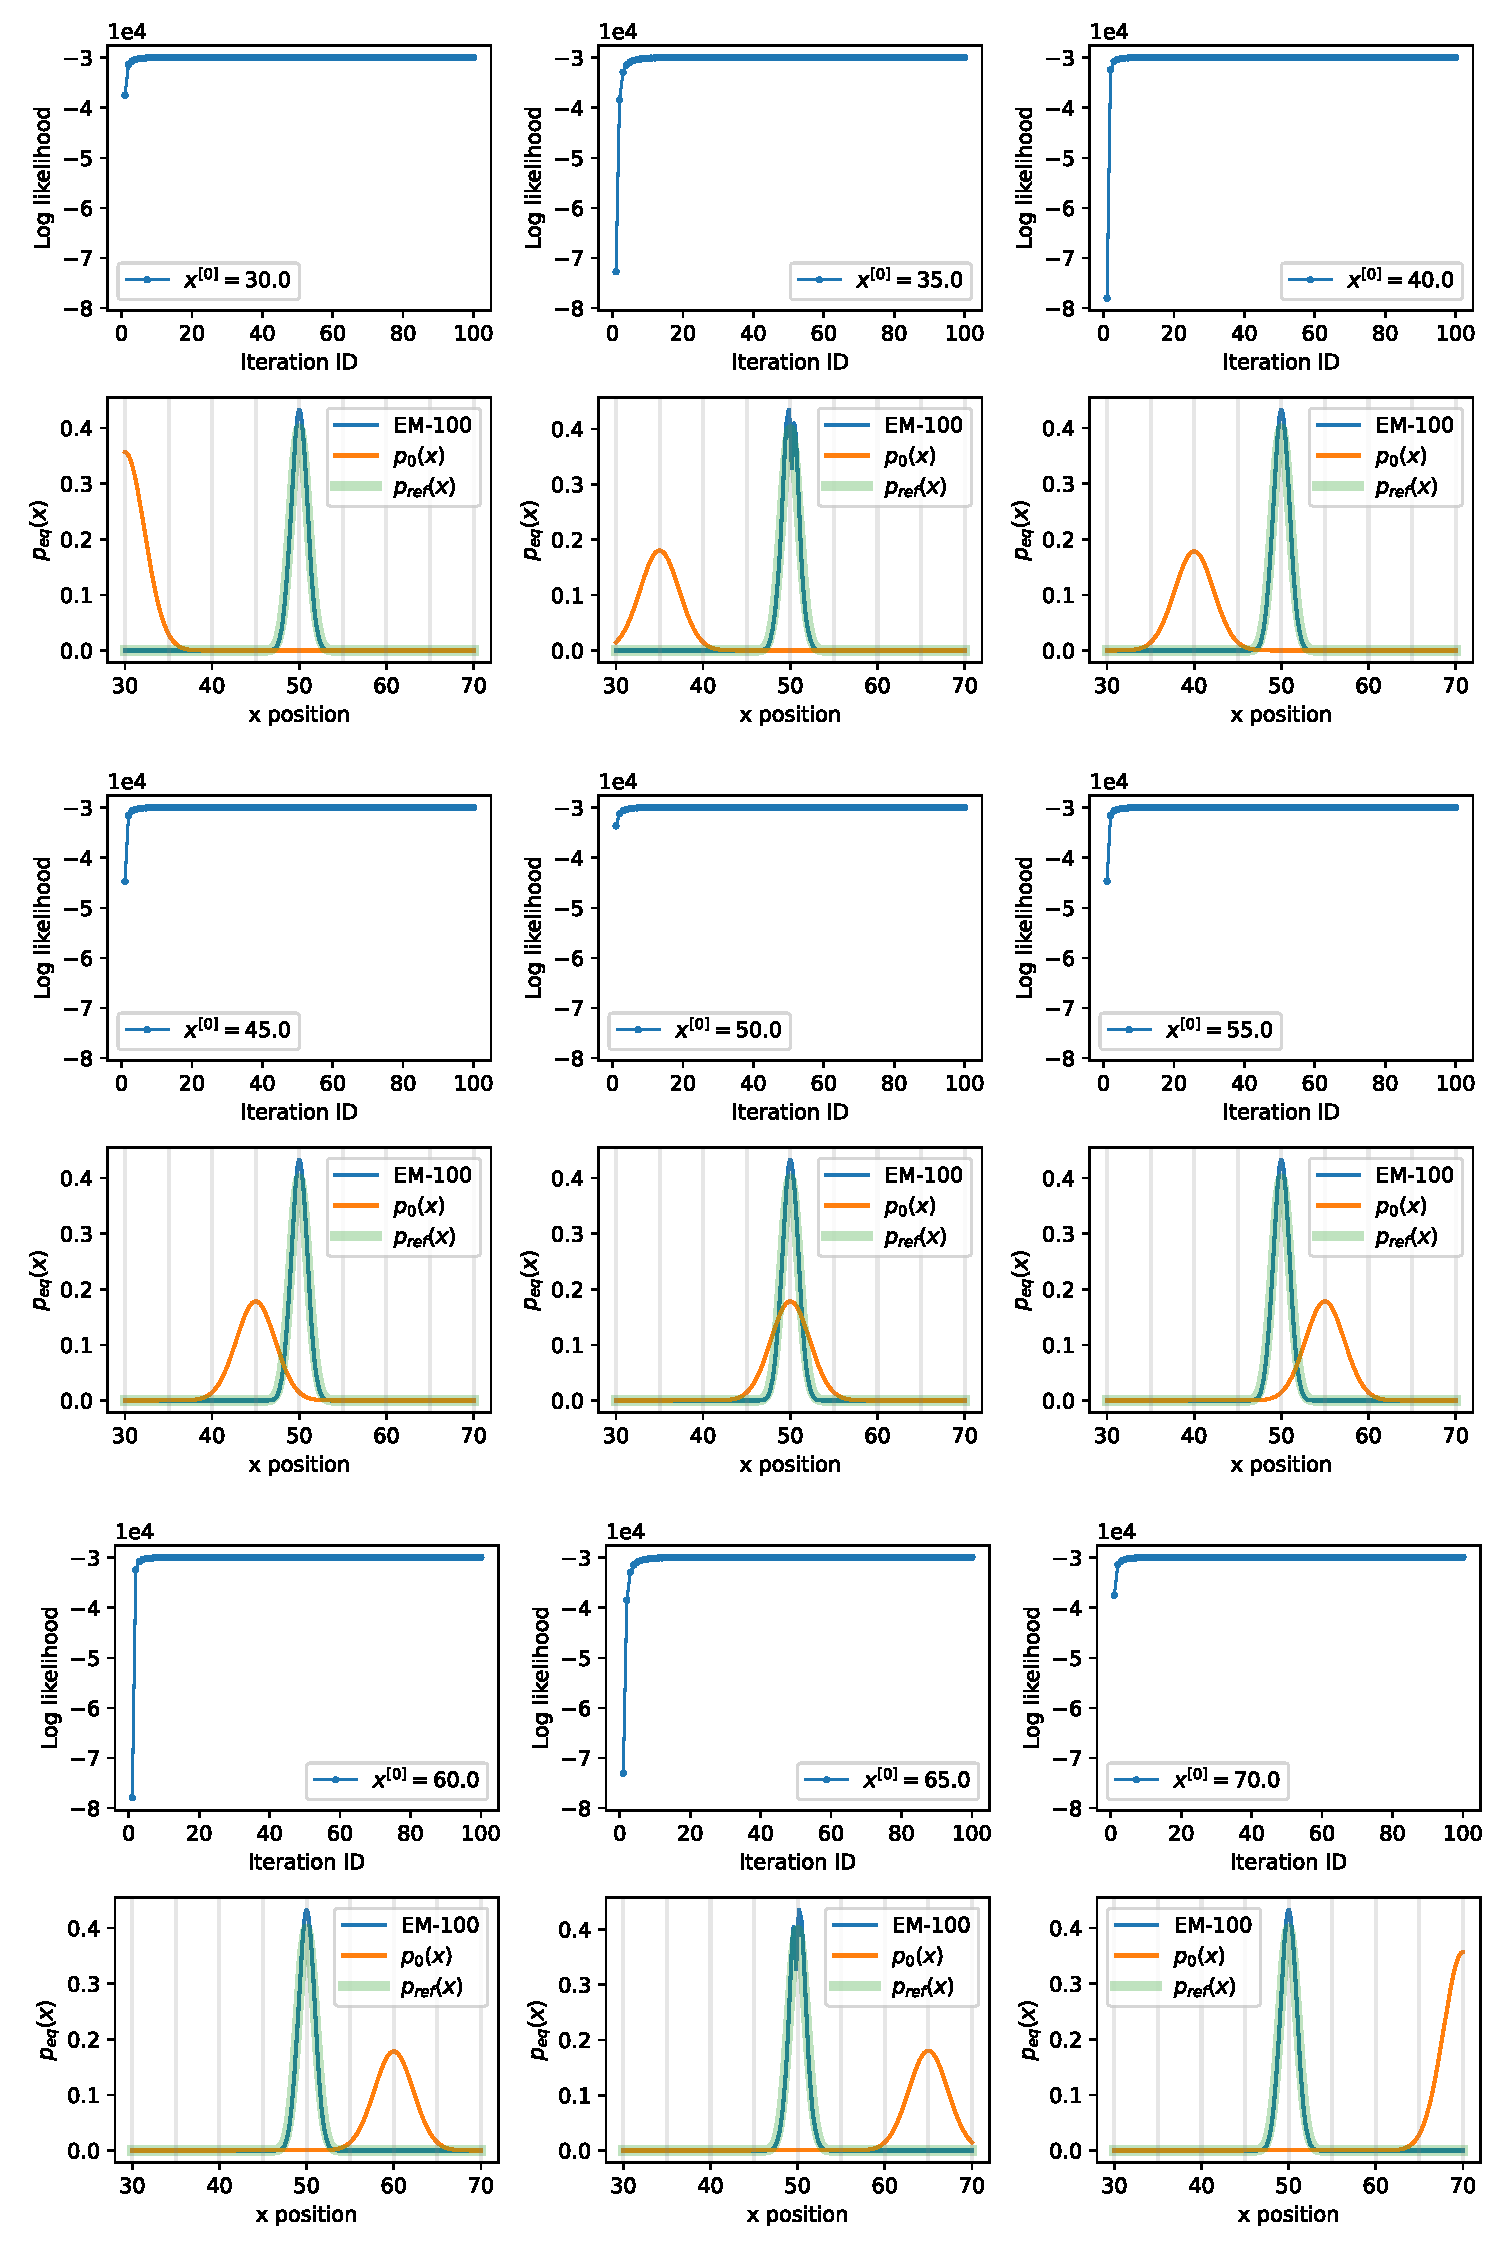
\includegraphics[scale=0.55]{ch4/initial_guess_test.pdf}   
\end{center}

\subsection{Troubleshooting: Double Peak}
\begin{center}
    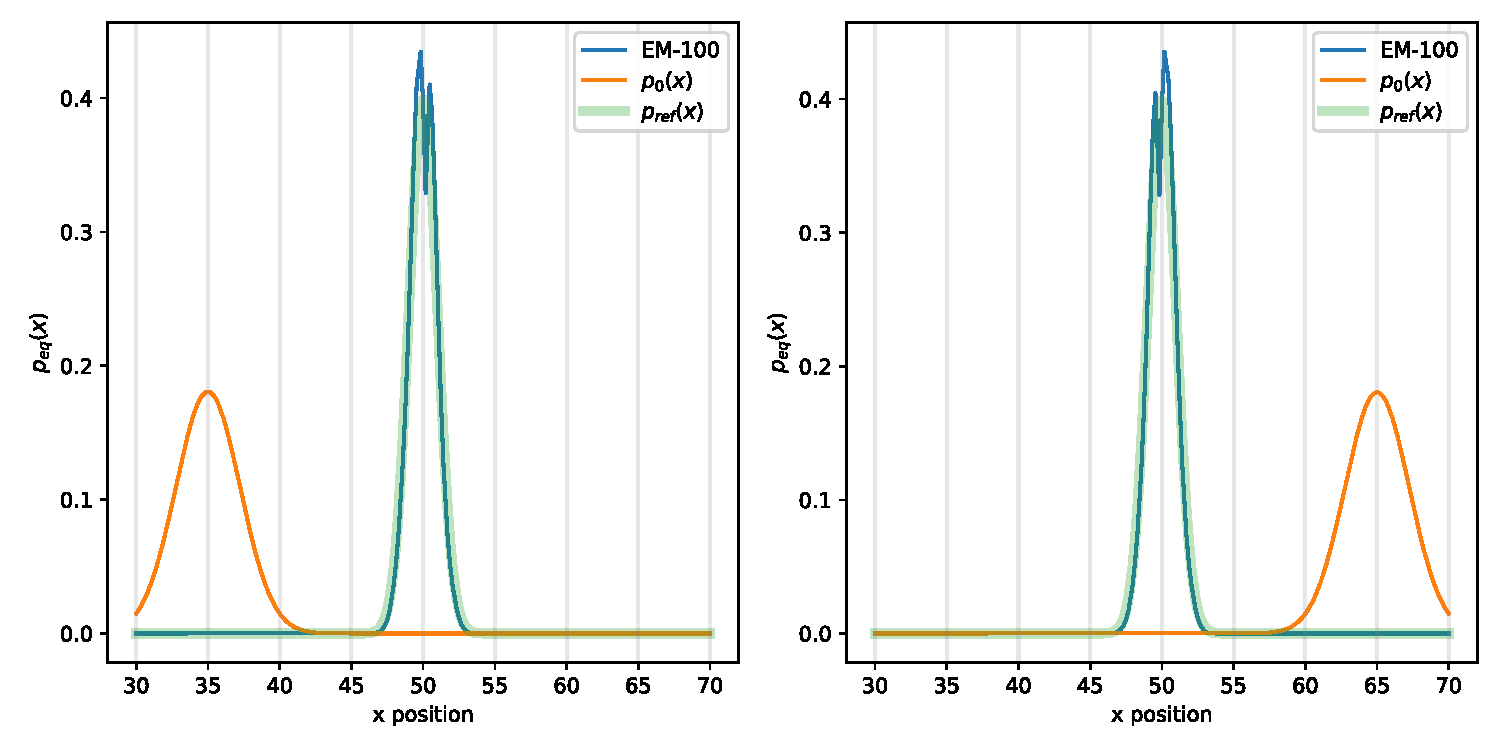
\includegraphics[scale=0.55]{ch4/double_peak_problem.pdf}   
\end{center}
\subsubsection{Step 1: Detect abrupt change}
\begin{itemize}
    \item Use finite difference to get $\frac{d p^{[k]}_{eq}(x)}{dx}$ and $\frac{d^2 p^{[k]}_{eq}(x)}{dx^2}$
    \item If $|\frac{d^2 p_{eq}(x)}{dx^2}|>1$, put the point into the list storing "change points"
    \item If $\text{Number}(\text{Change points}) > 0$, do smoothing. Else: no smooth 
\end{itemize}
\begin{center}
    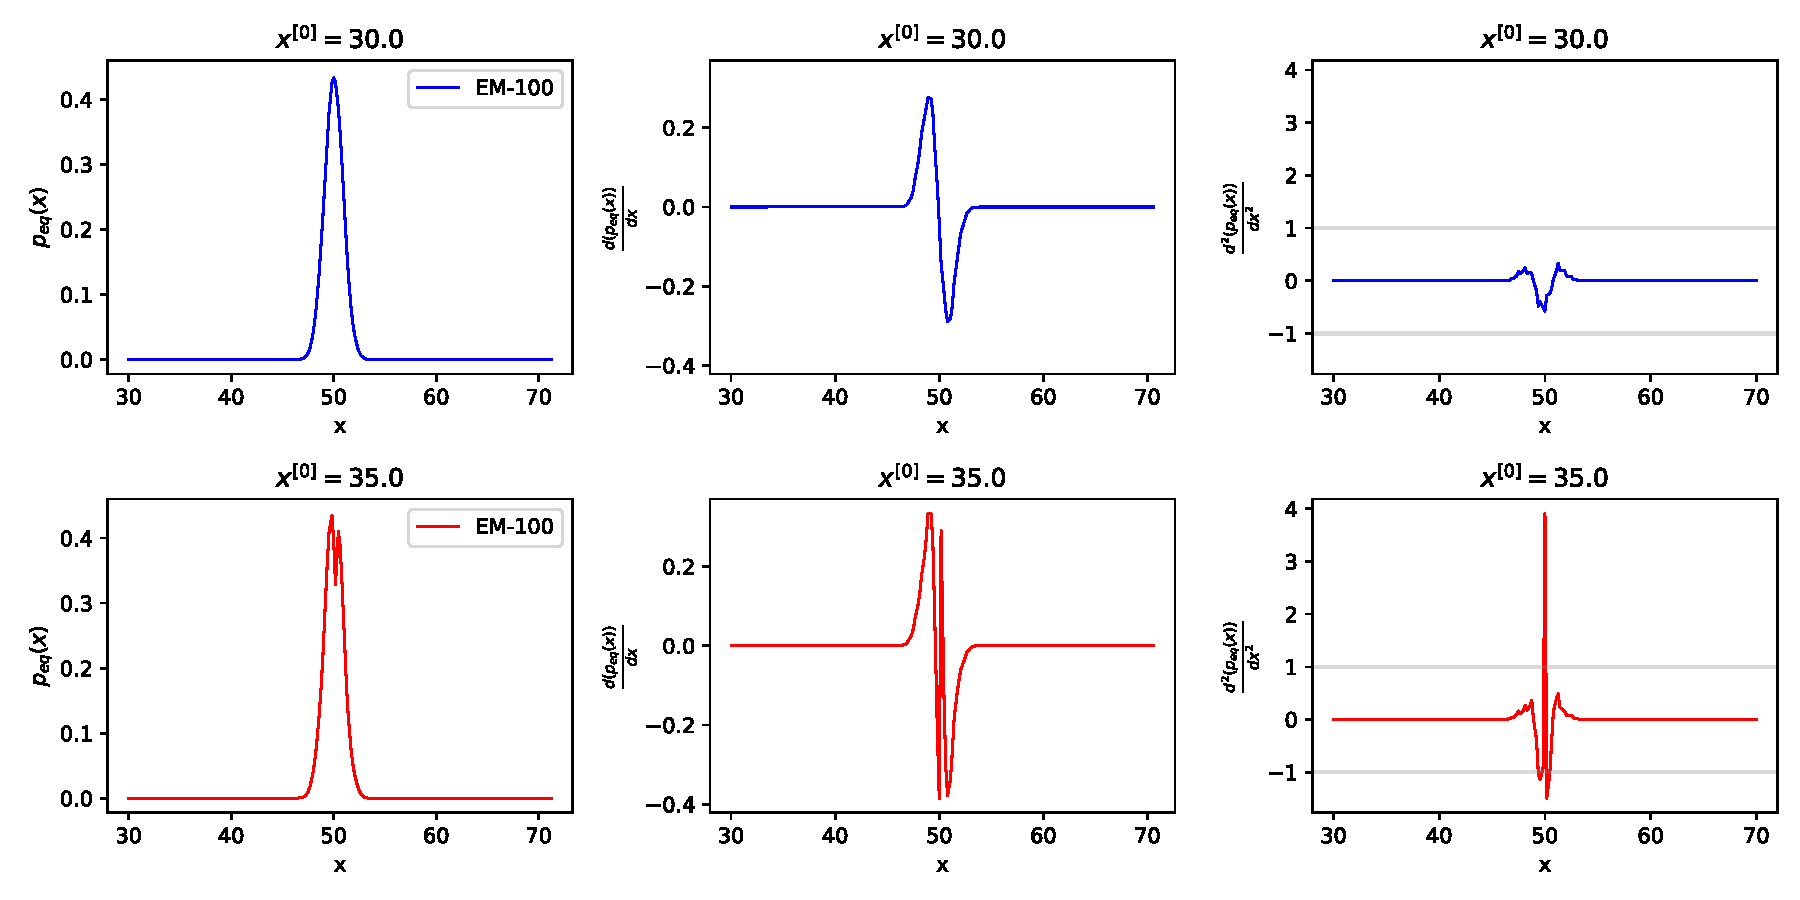
\includegraphics[scale=0.4]{ch4/double_peak_problem_derivative.pdf}   
\end{center}
\begin{center}
    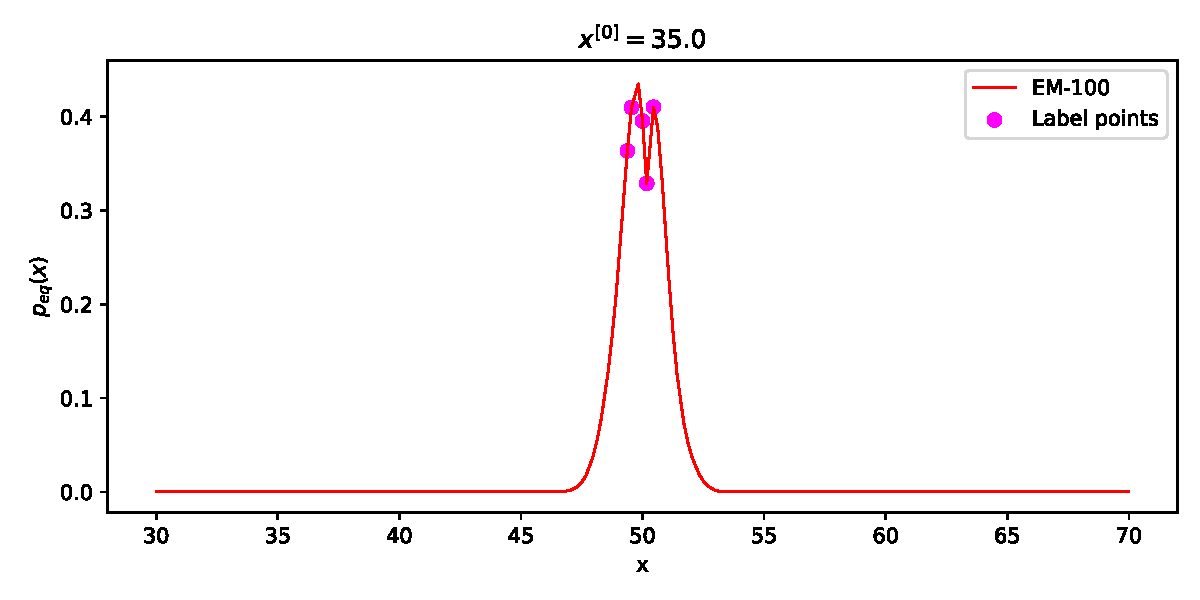
\includegraphics[scale=0.5]{ch4/abrupt_detect.pdf}   
\end{center}

\subsubsection{Step 2: The cubic smoothing spline}
\begin{definition}[Smoothing Spline]
    Let  $\{x_{i},Y_{i}:i=1,\dots ,n\}$ be a set of observations, modeled by the relation $\{Y_{i}=f(x_{i})+\epsilon _{i}\}$ where the $\epsilon _{i}$ are independen, zero mean random variables (usually assumed to have constant variance). The cubic smoothing spline estimate $\hat{f}$ of the function $f$ is defined to be the minimizer (over the class of twice differentiable functions) of
    \begin{equation}
         \sum _{i=1}^{n}\{Y_{i}-{\hat {f}}(x_{i})\}^{2}+\lambda \int {\hat {f}}''(x)^{2}\,dx
    \end{equation}
    \begin{itemize}
        \item $\lambda \geq 0$ is a smoothing parameter, controlling the trade-off between fidelity to the data and roughness of the function estimate. This is often estimated by generalized cross-validation, or by restricted marginal likelihood (REML) which exploits the link between spline smoothing and Bayesian estimation (the smoothing penalty can be viewed as being induced by a prior on the $f$.
        \item As $ \lambda \to 0$, the smoothing spline converges to the interpolating spline.
        \item As $\lambda \to \infty$(infinite smoothing), the roughness penalty becomes paramount and the estimate converges to a linear least squares estimate.
    \end{itemize}
\end{definition}
\begin{center}
    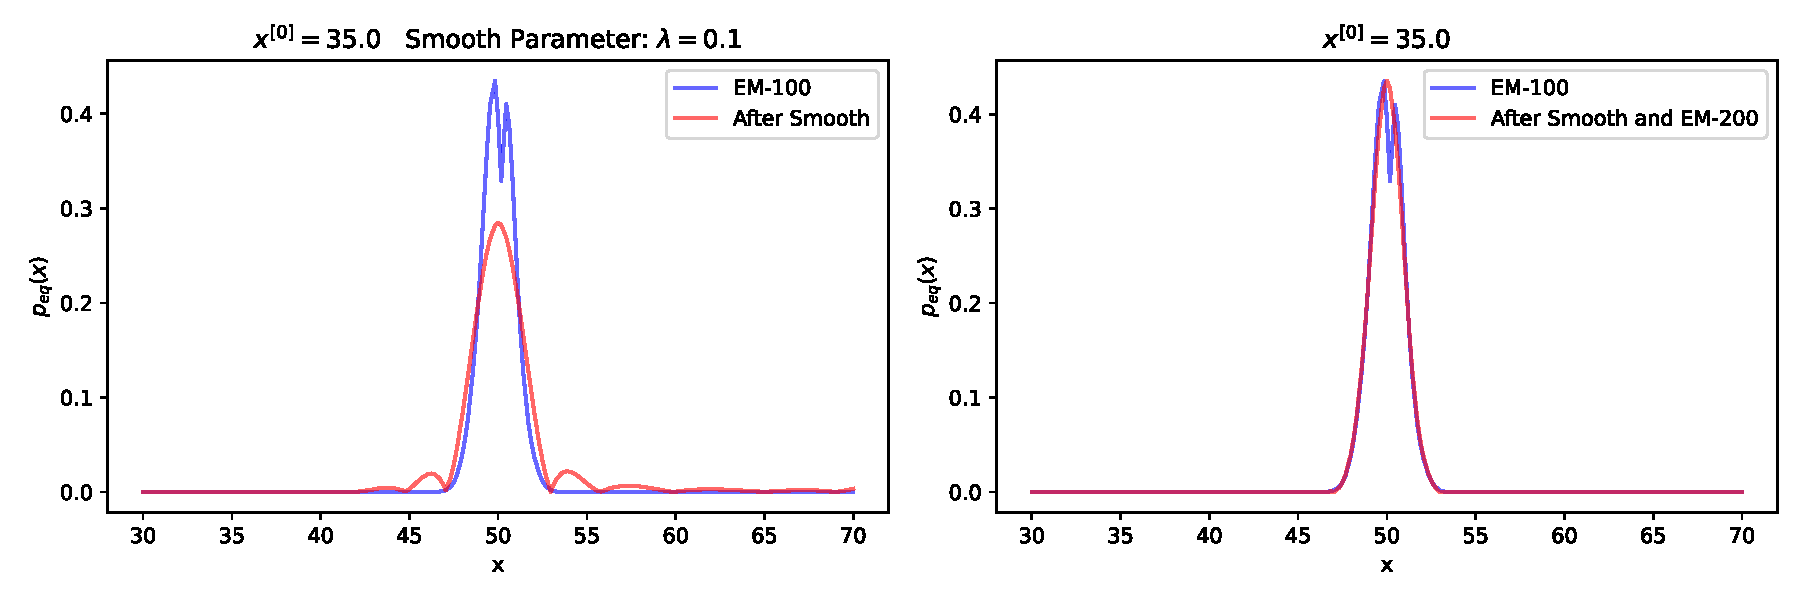
\includegraphics[scale=0.45]{ch4/double_peak_smooth_afterEM.pdf}   
\end{center}

\subsubsection{Result}
\begin{center}
    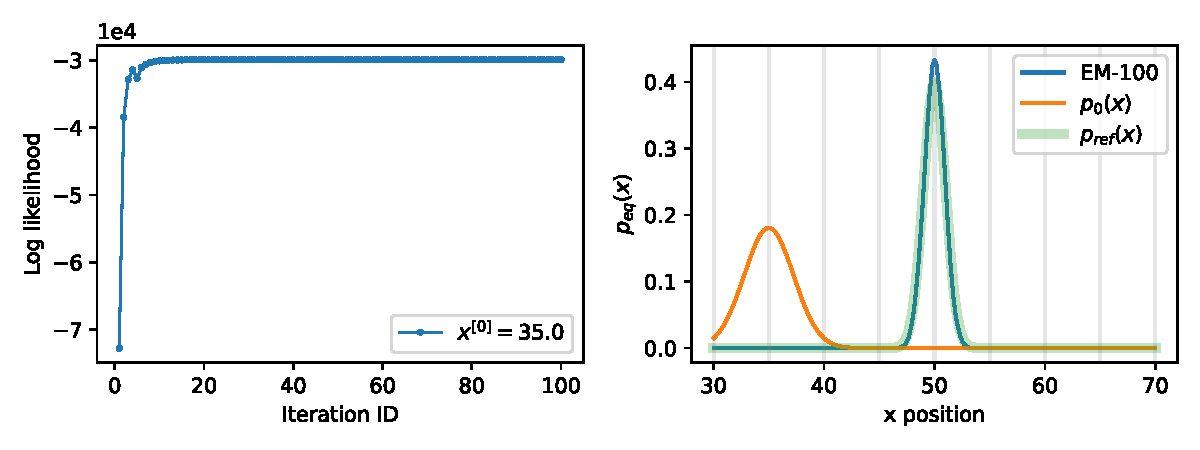
\includegraphics[scale=0.6]{ch4/aftersmooth_result.pdf}   
\end{center}

\section{Optimize diffusion coefficient D}
Here, we use the following simulation data to understand the procedure of updating D.
\begin{center}
    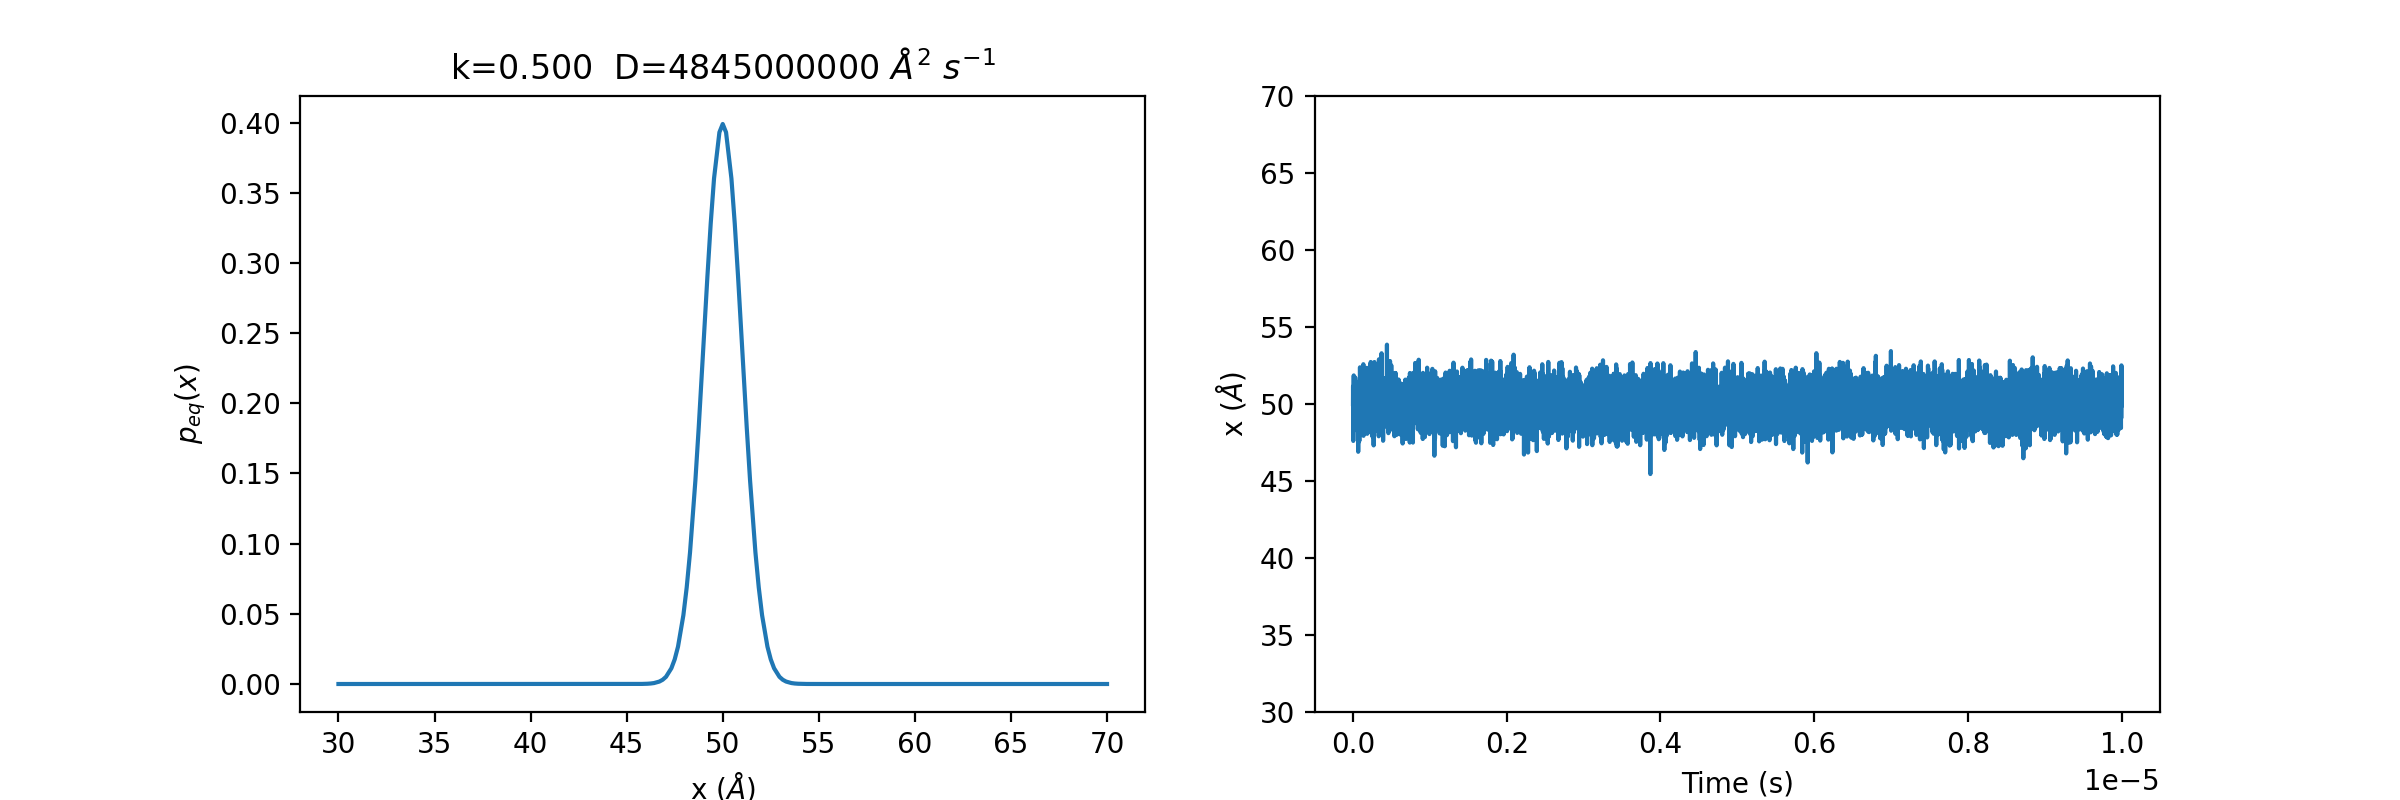
\includegraphics[scale=0.45]{ch4/Simu_for_EM.png}   
\end{center}
We will fix $p_{eq}^{[k]}$ as the real answer $p_{eq}$, and change $D$ to see the effect to eigenvalues $\lambda_i$ and log-likelihood $l[\theta]$

\subsection{Hamiltonian and its eigenvalues scale linearly with diffusion coefficient}
\begin{align*}
    \frac{\partial \rho(x,t)}{\partial t} &= -\bm{H}^0 \rho(x,t), \\
    \bm{H}^0 &= -D\nabla^2  + V_{\rm eff}(x), \\
    V_{\rm eff}  &= \frac{DF'(x)}{2} + \frac{DF^2(x)}{4}.
\end{align*}
\begin{center}
    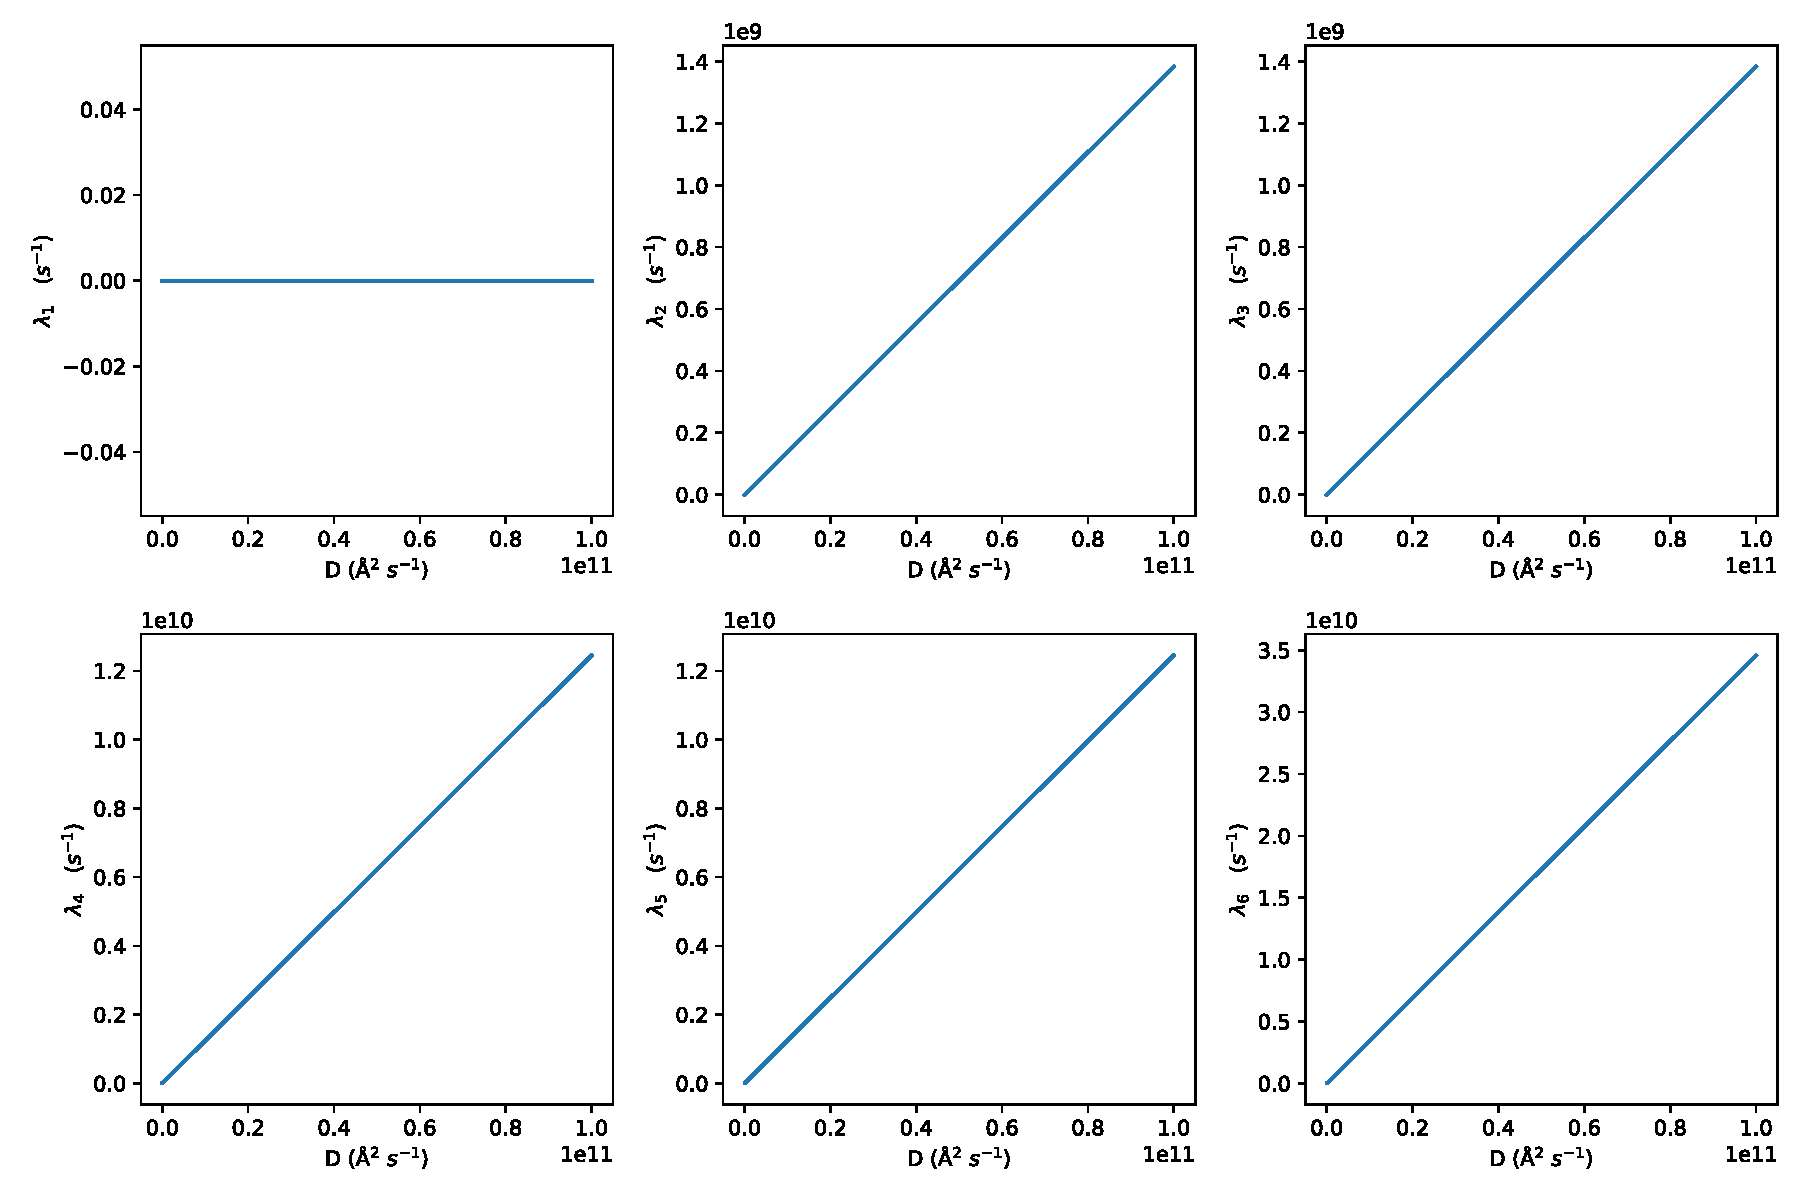
\includegraphics[scale=0.45]{ch4/eigenvalue_linear_with_D.pdf}   
\end{center}
I only show the first six eigenvalues, all the rest eigenvalues is linear scaling with $D$.

\subsection{Log-likelihood as a function of D}
First, I try 
\begin{align*}
    D = 10^{m}~\si{\angstrom}^{2}s^{-1}\text{   where } m=-2,...,11
\end{align*}
\begin{center}
    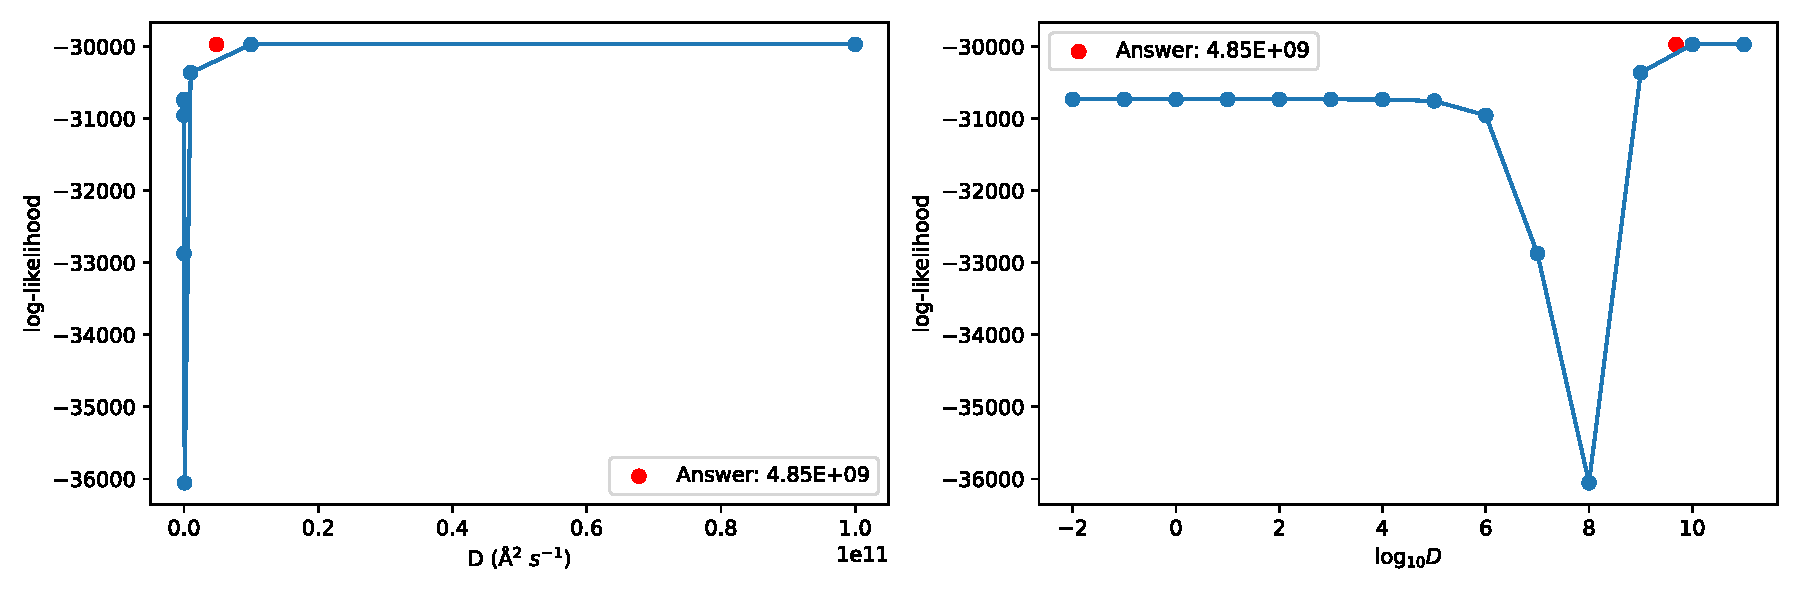
\includegraphics[scale=0.45]{ch4/D_loglikelihood_broad_search.pdf} 
\end{center}
Then, focus on the range from $1 \times 10^{8}$ to $9 \times 10^{9}$
\begin{center}
    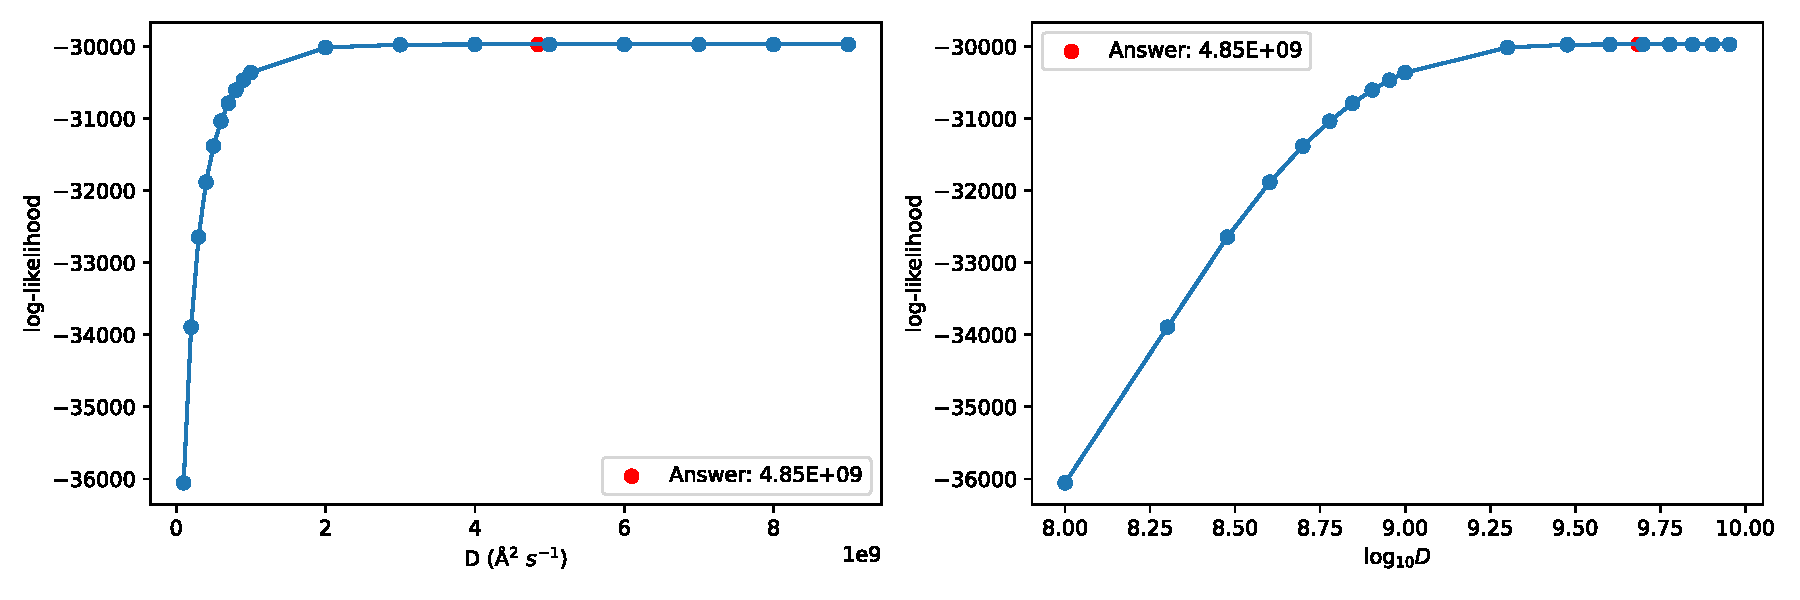
\includegraphics[scale=0.45]{ch4/D_loglikelihood_middle_search.pdf}   
\end{center}
At last, I focus on the range from $1.1 \times 10^{9}$ to $9.9 \times 10^{9}$
\begin{center}
    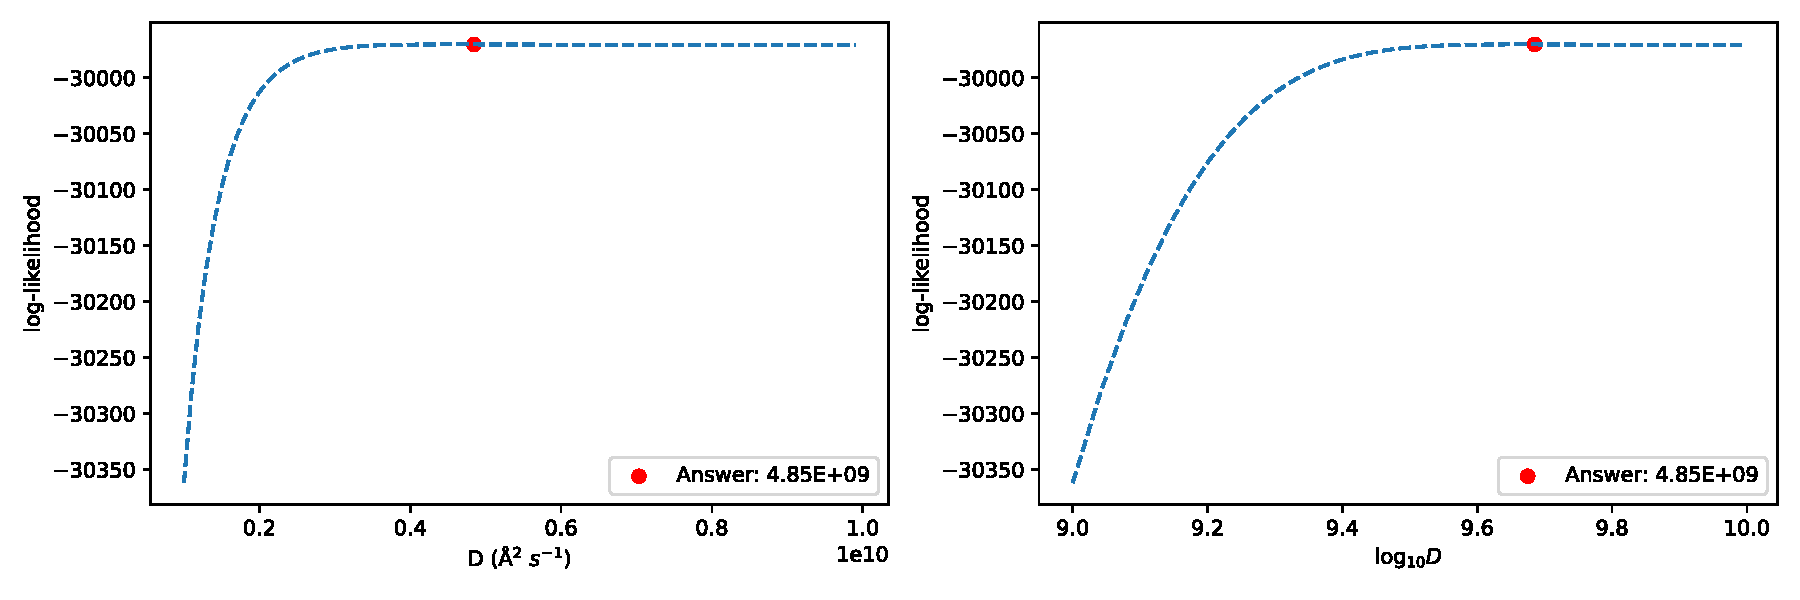
\includegraphics[scale=0.45]{ch4/D_loglikelihood_detail_search.pdf}   
\end{center}

\section{Complete EM}
\subsection{Initial Guess by Gaussian Kernel Density Estimation}
\begin{center}
    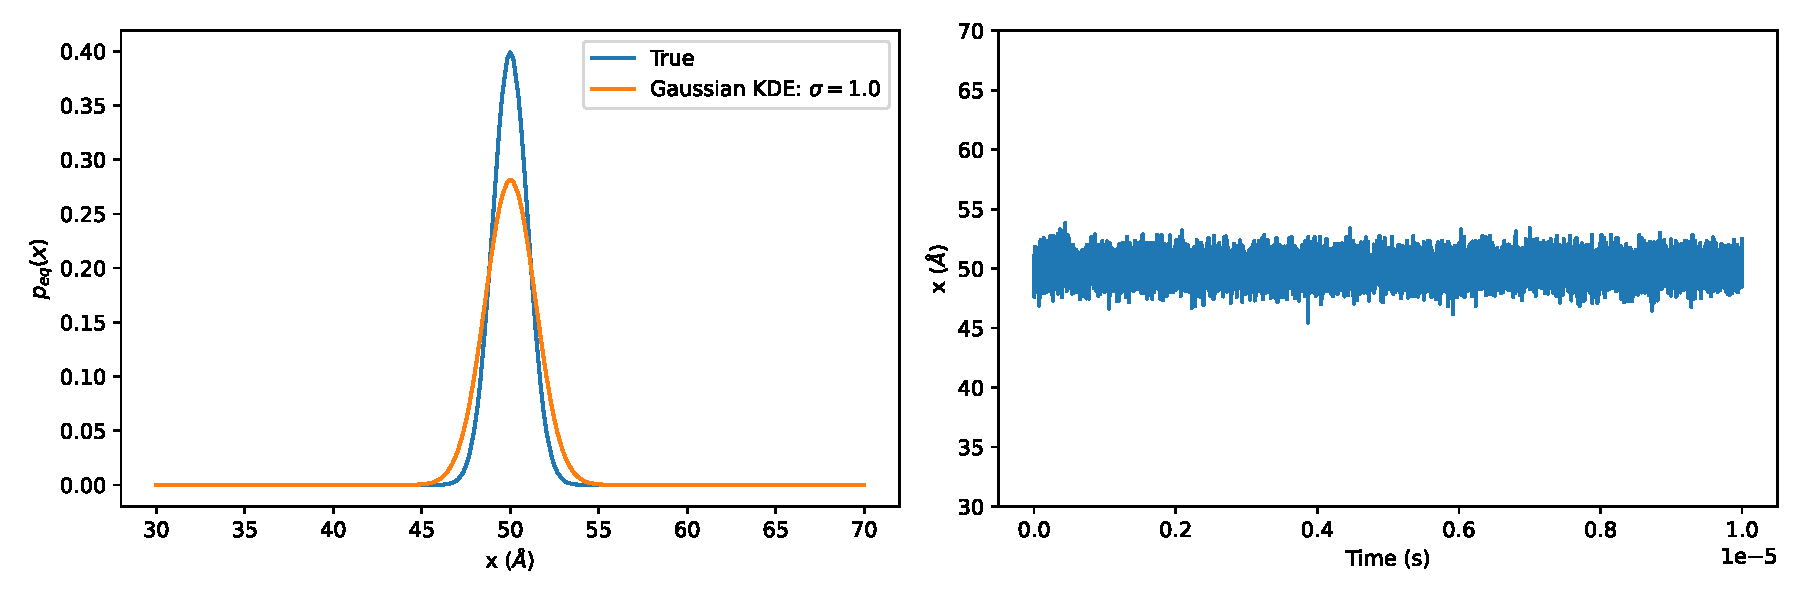
\includegraphics[scale=0.45]{ch4/Gaussian_Kde_harmonic_well.pdf} 
\end{center}

\subsection{Algorithm}
\begin{algorithm}[H]
    \SetAlgoLined
    \KwResult{$p^{k}_{\rm eq}$, $D^k$}
     initialize $p^0_{\rm eq}$ as Gaussian KDE \;
     initialize $D^0=\frac{k_B T}{6\pi \eta a}$\;
     
     \While{$(\ell[\theta^k] - \ell[\theta^{k-1}] > \num{1e-1})$ \& $(k < k_{\text{max}})$}{
       Eigen-decompose the Hermitian $\bm H$ for $\Psi$ and $\Lambda$\;
       Evaluate $\ell [\theta^k] = \sum_{\tau} |\alpha_{\tau}|$ via normalization\;
       Infer the latent states $\langle \alpha(t)|,|\beta(t) \rangle$\;
       Collect statistics of $\mathbb{E}^k_{X|Y}[a_ib_j] = \sum_{\tau}\Gamma^{\tau}_{ij}$\;
       Update $p_{\rm{eq}}^{k+1} = p^k_{\rm{eq}}(x) \sum_{ij} \mathbb{E}^k_{X|Y}[a_ib_j] \phi_i(x)\phi_j(x) $\;
       %
      \If{$k~\%~ 5 == 0$}{
       Detect abrupt change in $p^{k+1}_{\rm eq}$\;
       \If{abrupt change exists}{
           $p^{k+1}_{\rm eq}$ = Smooth($p^{k+1}_{\rm eq}$) 
       }
       Line search $D^{k+1} = \argmax_D \ell[p^{k+1}_{\rm eq},D]$\;
       }
       k = k + 1\;
     }
     \caption{Expectation-Maximization Statistical Learning for $F(x)$ and $D$}
\end{algorithm}

\subsection{The data strucutres for storing results}
\begin{align*}
    \mathrm{p\_container} &= 
    \begin{bmatrix}
        p^{0}_{\rm eq} \\ p^{1}_{\rm eq} \\ \vdots \\ p^{k}_{\rm eq}
    \end{bmatrix}\\
    \mathrm{D\_records} &= 
    \begin{bmatrix}
        D^{0} \\ D^{1} \\ \vdots \\ D^{k}
    \end{bmatrix}\\
    \mathrm{log\_likelihood\_records} &= 
    \begin{bmatrix}
        \ell[\theta^{0}] \\ \ell[\theta^{1}] \\ \vdots \\ \ell[\theta^{k}]
    \end{bmatrix}   
\end{align*}

\subsection{Results}
\begin{center}
    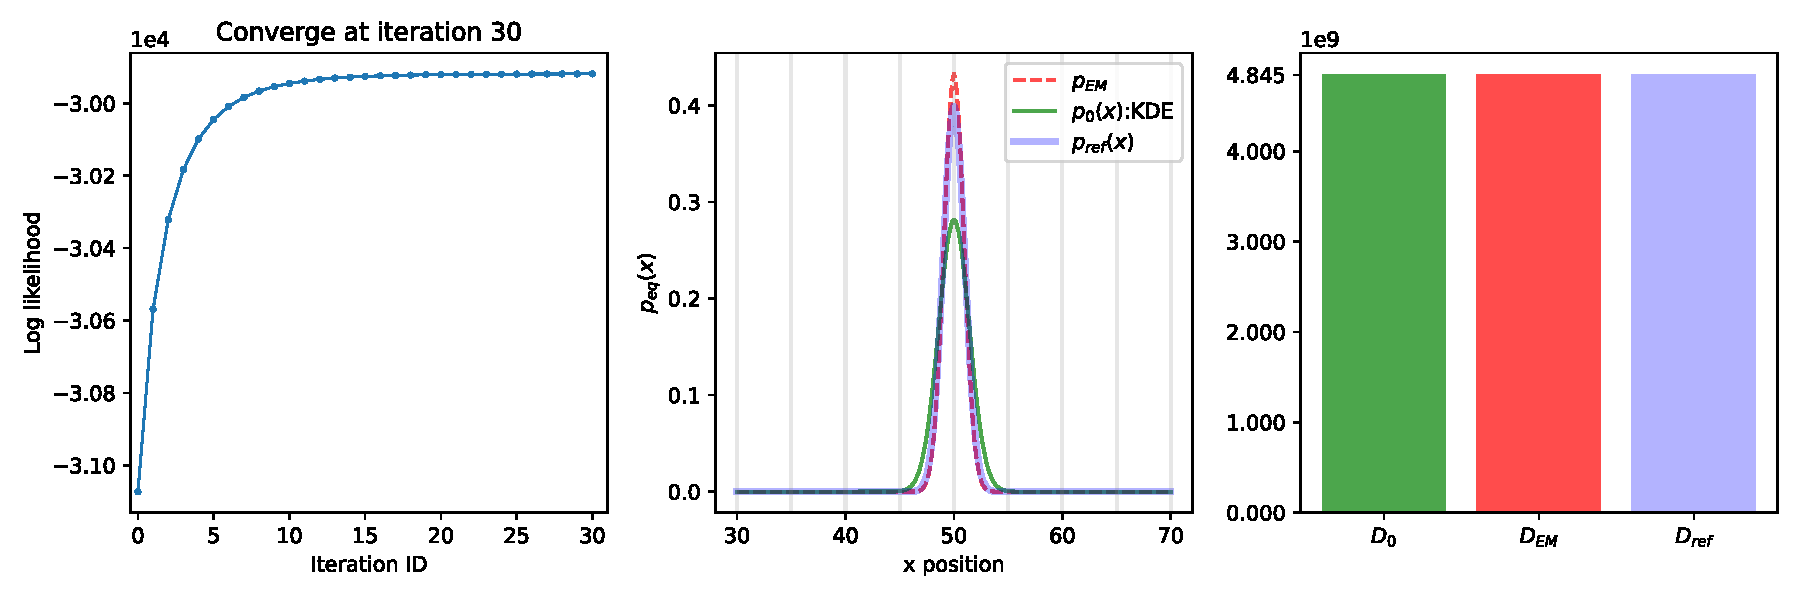
\includegraphics[scale=0.45]{ch4/em_p0_kde_pref_xavg_50.pdf} 
\end{center}

\section{Regularization by using Trajectory Entropy}
The proposed statistical learning problem of Langevin dynamics from smFRET data is naturally underdetermined because we attempt to extract a continuous profile from a finite number of photons. A Bayesian prior is thus required to break the degeneracy in the parameter set. With the prior, the posterior function, $p(\theta | \textbf{y})$, for parameter optimization becomes
\begin{equation}
    p(\theta | \textbf{y}) = \frac{p(\textbf{y}|\theta) p(\theta)}{p(\textbf{y})}
\end{equation}
A criterion for choosing the prior is to guide the optimization toward $F(x)$ profiles that imply the least amount information of dynamics. The goal is to prevent the statistical learning from overfitting and overinterpreting the measured data. As such, we selet the prior based on maximum trajectory entropy. For Langevin dynamics at equilibrium, the trajectory entropy is 
\begin{equation}
    \textbf{S}[F(x), D; D] = S_{\rm eq} - t_{\rm obs} \frac{D}{4}\left< F^2(x)\right>
\end{equation}
In Kevin's EM 2013 JPCB paper,
\begin{align}
    D &= 500~~\text{s}^{-1} \\
    \eta_{F} &= 2 \times 10^{-7} \\ 
    \eta_{F}D &= 0.0001
\end{align}
Therefore, when including the prior for updating $p_{\rm eq}$
\begin{align*}
    p_{\rm eq}^{k+1}(x) &= \left(\mathbb{E}^k_{X|Y} \left[\delta(x-X) \right]\right)^{1/(1+\eta_FD)} \\
    &= \left(\mathbb{E}^k_{X|Y} \left[\delta(x-X) \right]\right)^{1/(1+0.0001)} \\
    &= \left(\mathbb{E}^k_{X|Y} \left[\delta(x-X) \right]\right)^{1/(1.0001)}
\end{align*}
I think the regularization has no real effect.
